\chapter{Astrazione dei modelli}

Dato un \emph{fault model}, si procede con l'astrazione dei modelli mediante una qualche rappresentazione strutturale degli stessi.

Nel caso in esame, l'astrazione realizzata è il \emph{diagramma delle classi}, una rappresentazione che pone l'accento sulla struttura degli oggetti del sistema (classi di appartenenza, relazioni, attributi e operazioni).

Vengono qua riportati i diagrammi delle classi delle tre architetture in esame.

\begin{figure}[h] 
  \centering
    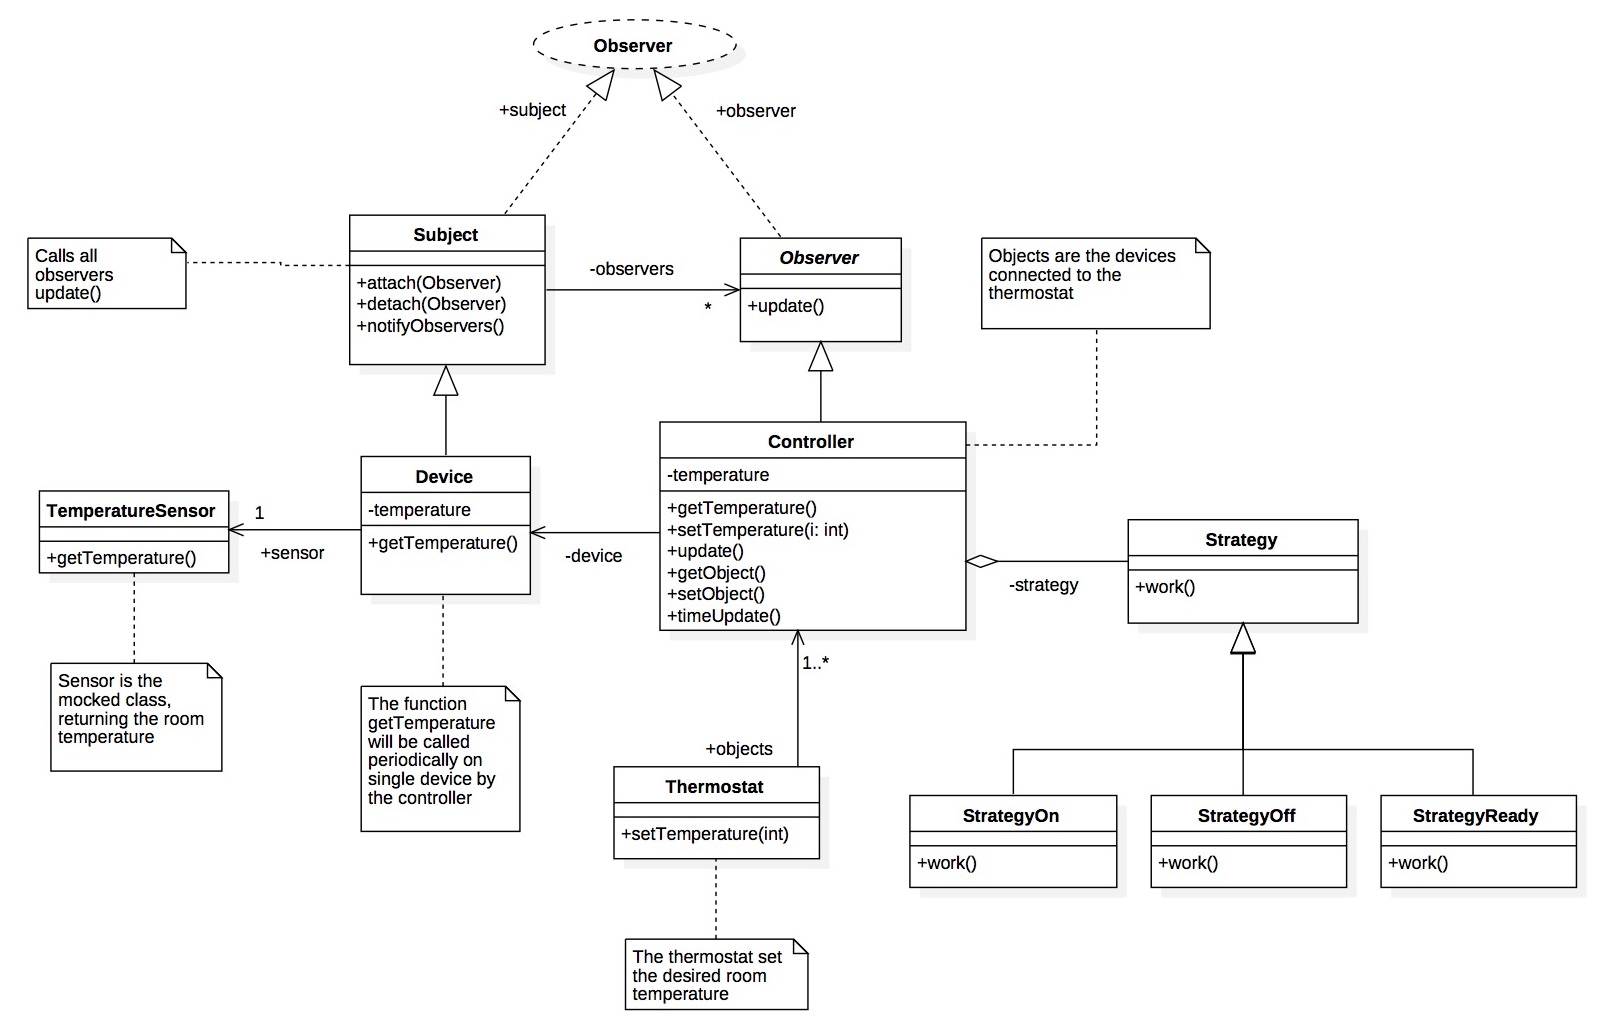
\includegraphics[width=1\textwidth]{ObserverStrategy.jpg}
    \caption{{\small \textit{Diagramma delle classi dell'architettura contenente l'Observer e lo Strategy, il Termostato}}}
\end{figure}

\begin{figure}[h] 
  \centering
    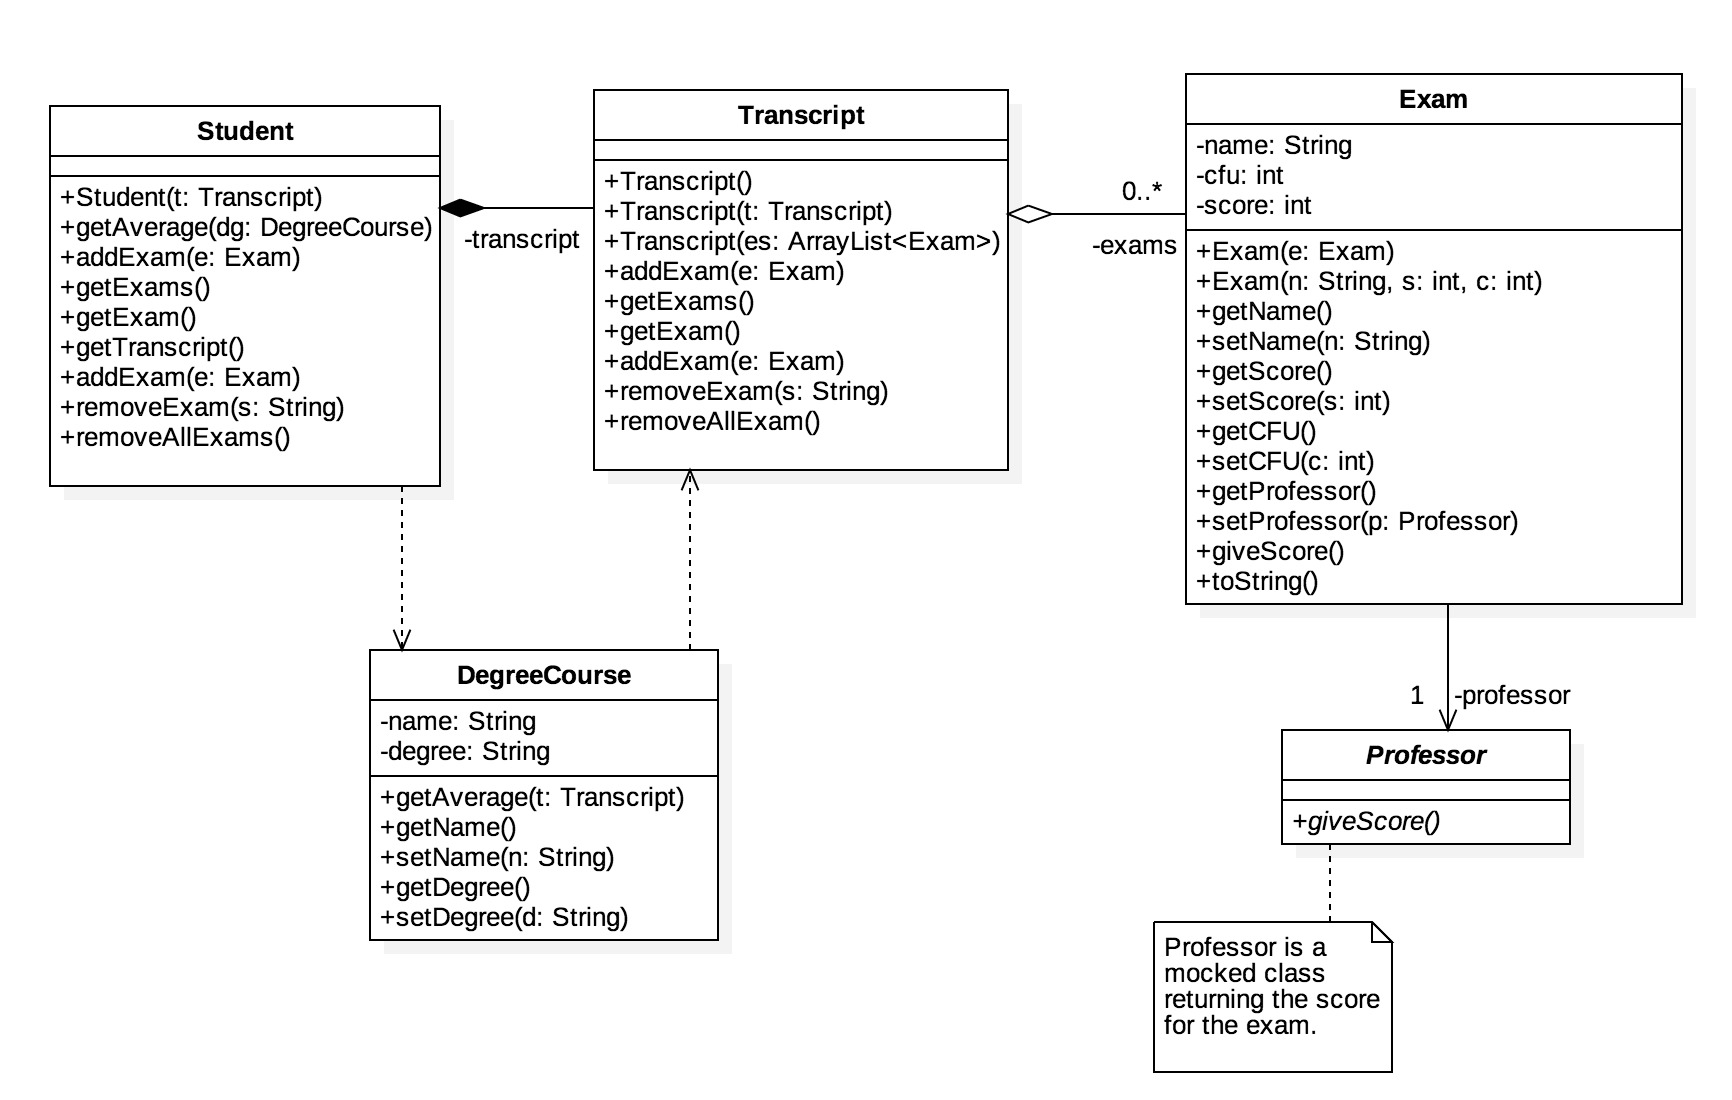
\includegraphics[width=1\textwidth]{defensivecopy.jpg}
    \caption{{\small \textit{Diagramma delle classi dell'architettura del sistema esami (copia difensiva)}}}
\end{figure}

\begin{figure}[h] 
  \centering
    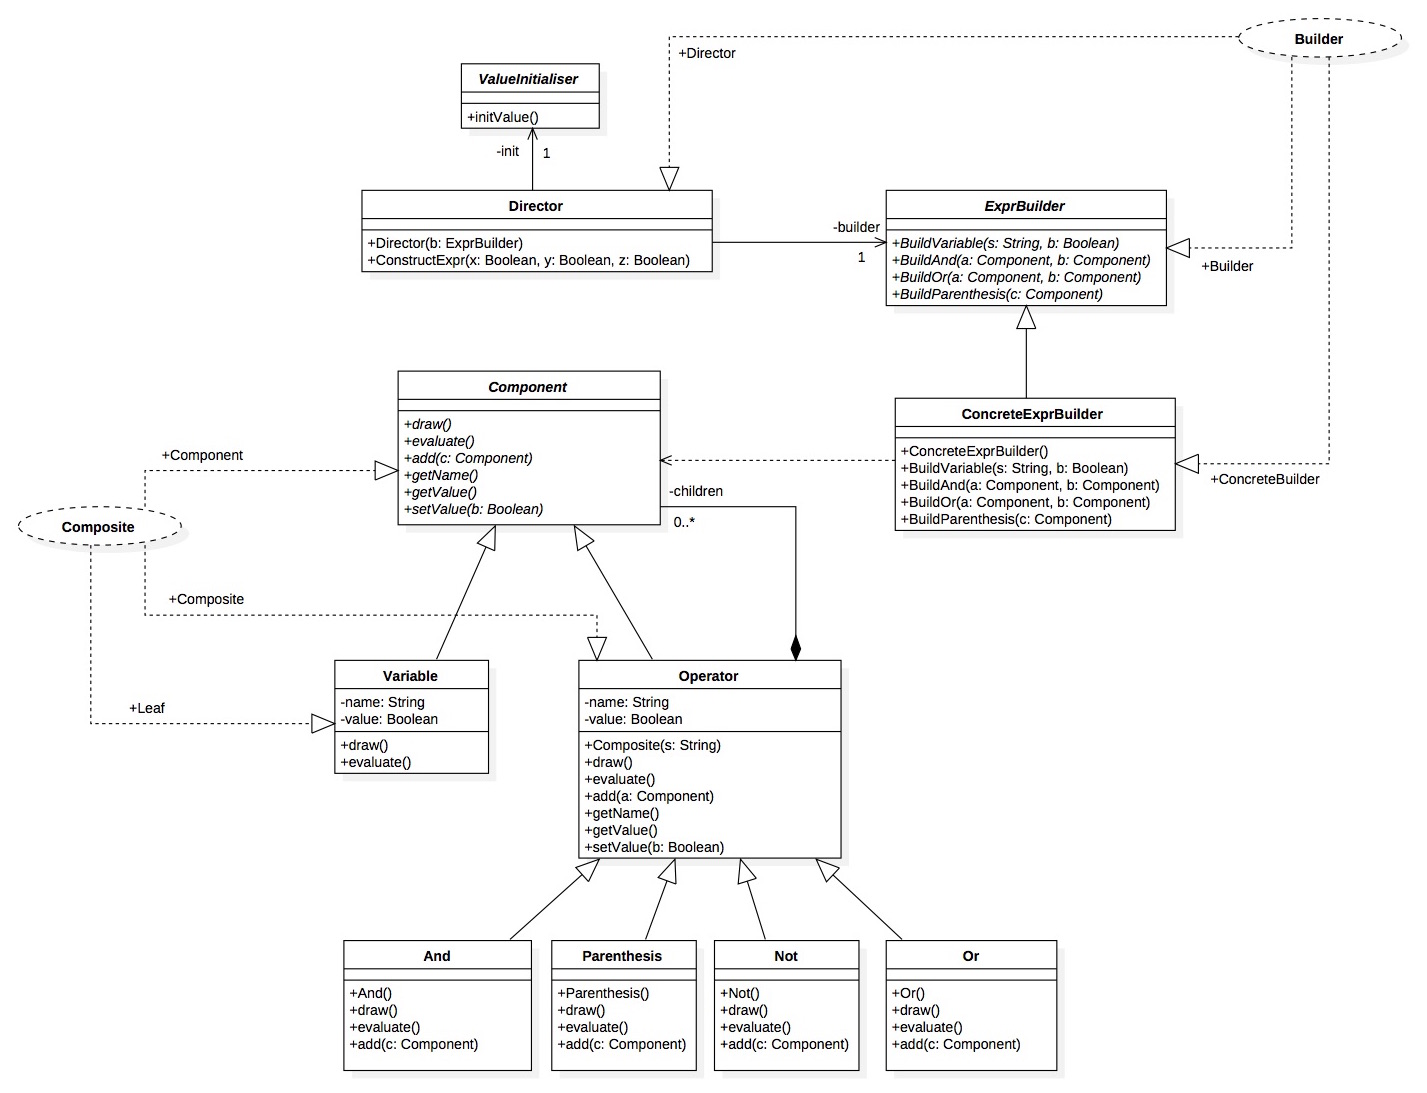
\includegraphics[width=1\textwidth]{buildercomposite.jpg}
    \caption{{\small \textit{Diagramma delle classi dell'architettura contenente il Builder ed il Composite, il generatore di espressioni booleane}}}
\end{figure}

Nel diagramma delle classi vengono inoltre evidenziati i \emph{design patterns} utilizzati mediante una serie di annotazioni dedicate. In questo modo è possibile focalizzare l'attenzione sulle criticità presenti nel \emph{fault model } e da questi dipendenti.

In aggiunta al diagramma delle classi sono stati poi realizzati anche tre diversi \emph{Control Flow Graph} rappresentanti tre casi d'uso tipici delle diverse architetture. 

\begin{figure}[h] 
  \centering
    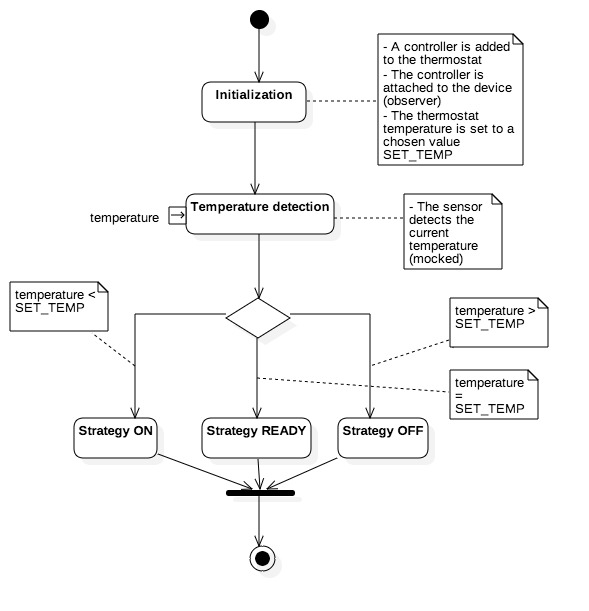
\includegraphics[width=0.7\textwidth]{observerstrategy-cfg}
    \caption{{\small \textit{Control Flow Graph del caso d'uso relativo all'attuazione della giusta strategia in base alla temperatura rilevata dal sensore nella prima architettura}}}
\end{figure}

\begin{figure}[h] 
  \centering
    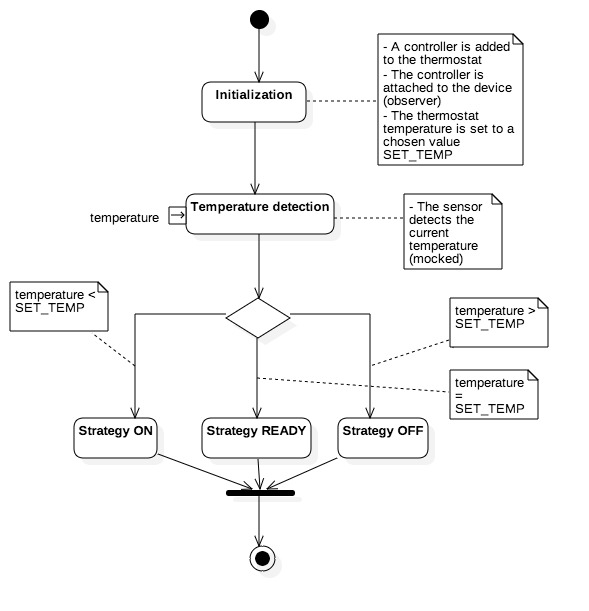
\includegraphics[width=0.7\textwidth]{defensivecopy-cfg}
    \caption{{\small \textit{Control Flow Graph del caso d'uso relativo all'assegnamento del voto ad un esame da parte di un professore ed il calcolo della media dei voti}}}
\end{figure}

\begin{figure}[h] 
  \centering
    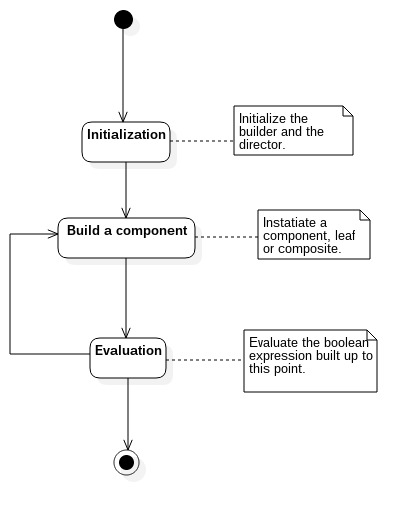
\includegraphics[width=0.7\textwidth]{buildercomposite-cfg}
    \caption{{\small \textit{Control Flow Graph del caso d'uso relativo alla creazione e valutazione di un'espressione booleana}}}
\end{figure}

Grazie all'astrazione del modello così rappresentata, è possibile proseguire andando a definire un criterio di copertura adeguato a verificare le criticità esposte nel \emph{fault model}.

